% this file is called up by thesis.tex
% content in this file will be fed into the main document

%: ----------------------- name of chapter  -------------------------
\chapter{Weryfikacja rozwiązania} % top level followed by section, subsection


%: ----------------------- paths to graphics ------------------------

% change according to folder and file names
\ifpdf
    \graphicspath{{4/figures/PNG/}{4/figures/PDF/}{4/figures/}}
\else
    \graphicspath{{4/figures/EPS/}{4/figures/}}
\fi

%: ----------------------- contents from here ------------------------

Rozdział ten jest podzielony na trzy części. Część pierwsza opisuje jak wybrany sposób integracji oraz powstały w ten sposób prototypowy system wpływa na łatwość tworzenia i efektywność aplikacji przetwarzających mowę. Proponowane przykładowe aplikacje to:
\begin{itemize}
	\item Automatyczne dyktando
	\item Lektor RSS
	\item Lektor SMS
	\item Konwerter plików graficznych do tekstowych
\end{itemize}
Każdej z proponowanych aplikacji poświęcono osobny podrozdział, w którym jest zdefiniowany przypadek użycia, przedstawione są wymagania funkcjonalne i niefunkcjonalne oraz przedstawiona jest weryfikacja podejścia. Część druga tego rozdziału opisuje testy (i ich wyniki) którym została poddana prototypowa implementacja systemu. Ostatnia część wynikające z części poprzednich.

\section{Weryfikacja funkcjonalności}
\subsection{Automatyczne dyktando}
Jest to aplikacja webowa umożliwiająca użytkownikowi ćwiczenie pisowni w różnych językach. Zasada działania jest bardzo prosta, użytkownik ładuje plik tekstowy lub graficzny na serwer oraz wybiera język docelowy, następnie zostaje przekierowany na stronę zawierającą formularz do pisania tekstu oraz odtwarzacz. Użytkownik słucha tekstu i zapisuje w polu tekstowym transkrypcję. W momencie w którym zatwierdzi formularz zostaje on przesłany na serwer i porównany z oryginalnym plikiem wejściowym, w efekcie użytkownik otrzymuje informację o ilości popełnionych błędów oraz o wyrazach które źle zapisał. 
\subsubsection{Przypadek użycia}
\begin{figure}[!h]
	\centering
	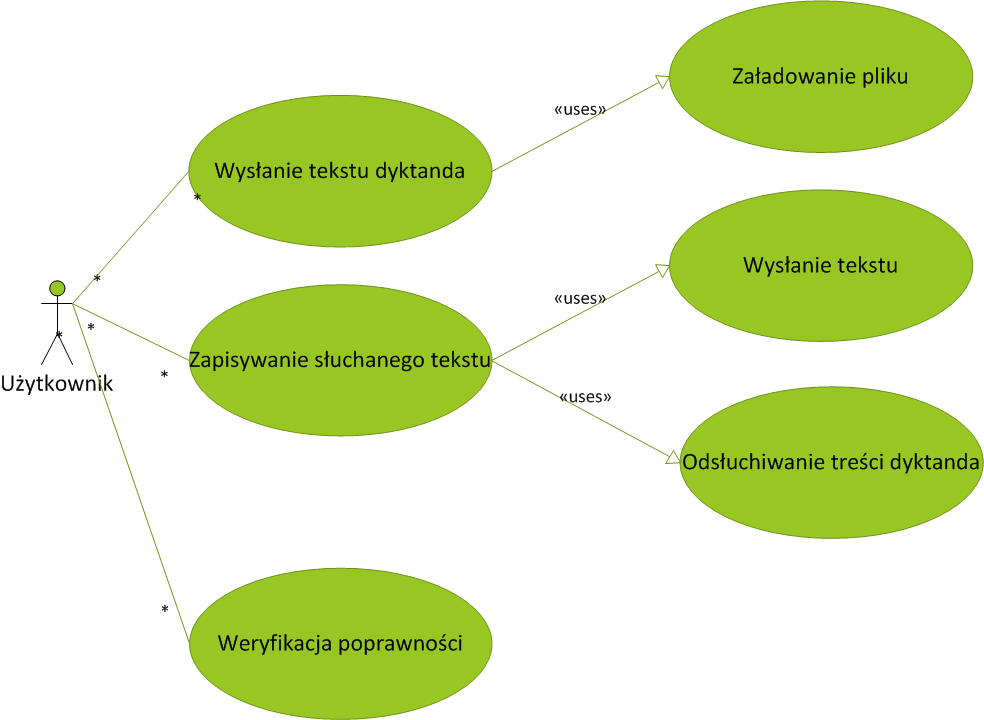
\includegraphics[scale=0.45]{useCaseDictando.png} 
	\caption{Przypadek użycia - Automatyczne dyktando }
\end{figure}


\subsubsection{Wymagania funkcjonalne}
\begin{enumerate}
	\item Obsługiwanie wielu języków
	\item Możliwość podania tekstu źródłowego
		\begin{enumerate}
			\item jako plik graficzny
			\item jako plik tekstowy, wysyłany na serwer
		\end{enumerate}
	\item Umożliwienie użytkownikowi odsłuchania wysłanego tekstu w wybranym przez niego języku
	\item Umożliwienie użytkownikowi wprowadzania tekstu jednocześnie z odsłuchiwaniem
	\item Wygenerowanie i wyświetlenie raportu o ilości błędów popełnionych przez użytkownika
\end{enumerate}

\subsubsection{Wymagania niefunkcjonalne}
\begin{enumerate}
	\item Bezpieczeństwo - użytkownik i tylko on powinien móc widzieć swoje wyniki
	\item Wydajność - dyktowanie tekstu powinno przebiegać płynnie, opóźnienie może występować tylko przed rozpoczęciem, od 0 do 60 sekund, przerwy w czasie dyktowania tekstu są niedopuszczalne
	\item Niezawodność - użytkownik powinien zawsze otrzymać wynik który jest poprawny, tzn. pokazuje dokładną ilość błędów popełnionych przez użytkownika
\end{enumerate}

\subsubsection{Weryfikacja podejścia}
Jak widać w powyższym podrozdziale wymagania stawiane przed aplikacją są precyzyjne i klarowne. Zastosowane podejście integracyjne sprawia, że stworzenie aplikacji spełniającej wymagania staje się proste. Zapewnienie obsługi wielu języków nie wymaga praktycznie żadnego nakładu pracy ze strony programisty aplikacji klienckiej. Jak zostało to opisane w rozdziale drugim, przy zastosowanym podejściu wystarczy wygenerować i przesłać plik xml z informacją dotyczącą języka docelowego, działa to niezależnie od języka w którym jest tekst wejściowy (pod warunkiem, że w pliku konfiguracyjnym ustawi się tag odpowiedzialny za usługę rozpoznającą język). Podobnie przesłanie pliku graficznego, również wymaga tylko umieszczenia odpowiedniego tagu w pliku xml celem wywołania usługi OCR. Jak łatwo zauważyć wygenerowanie i przesłanie pliku xml nie jest dużym wyzwaniem programistycznym.Widać to szczególnie gdyby porównać to z implementacją bez wykorzystania systemu opartego o rozwiązanie opisane w tej pracy. Musiałaby ona łączyć się z kilkoma zewnętrznymi usługami, z których każdy prawdopodobnie miałby inny interfejs, konwertować różne formaty plików, obsługiwać błędy itd. Jak widać, w tym przypadku, zastosowane podejście w sposób znaczący pozytywnie wpływa na łatwość i szybkość implementacji aplikacji klienckiej, co więcej sprawia ono, że w przyszłości aplikacja może zostać rozbudowana lub też łatwo przeniesiona na inne platformy np. telefony. \\

\subsection{Lektor SMS}
Jest to aplikacja przeznaczona dla systemu operacyjnego Android. Jak nazwa wskazuje jej funkcjonalność pozwala odczytywać na głos wiadomości tekstowe. Może okazać się bardzo przydatna w czasie jazdy samochodem, wiadomo, że używanie telefonu komórkowego jest zabronione z powodu bezpieczeństwa, tym bardziej, używanie rąk i skupianie wzroku na odczytywanej wiadomości tekstowej jeszcze w większym stopniu niż rozmowa przez telefon prowadzi do odwrócenia uwagi kierowcy od sytuacji na drodze.
Zasada działania tej aplikacji jest bardzo prosta, mianowicie po włączenie przechwytuje ona każde zdarzenie oznaczające otrzymanie wiadomości tekstowej, pobiera jej treść i zamienia ją na dźwięk w dowolnym, wybranym przez użytkownika języku. Co warte zauważenia aplikacja ta ma dwa różne sposoby generowania mowy:
\begin{itemize}
	\item korzystając z usług udostępnianych przez przykładową implementację systemu integrującego usługi przetwarzania mowy
	\item korzystając z wbudowanej w system Android funkcjonalności TTS
\end{itemize} 
Dzięki wykorzystaniu obu rozwiązań mamy możliwość bezpośredniego porównania. Wybór sposobu generowania dźwięku zależy od dostępności połączenia z internetem, jeżeli takie istnieje to aplikacja korzysta z zewnętrznego systemu, w przeciwnym razie wykorzystuje wbudowany TTS. Oczywiście użytkownik ma możliwość ustawienia dla których numerów aplikacja będzie działać.
\newpage
\subsubsection{Przypadek użycia}
\begin{figure}[!h]
	\centering
	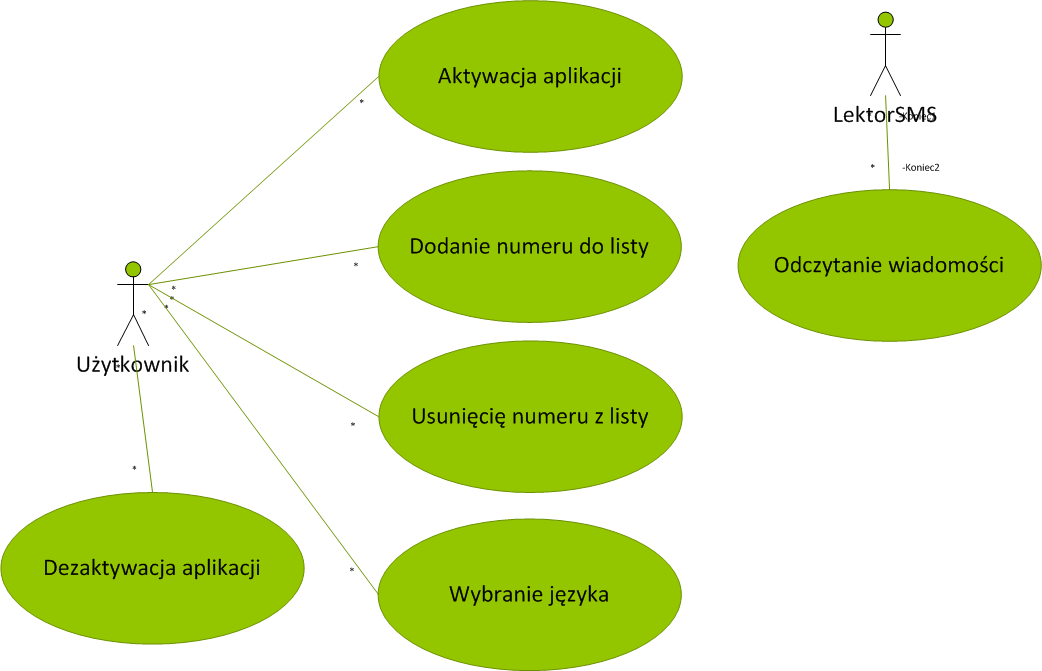
\includegraphics[scale=0.45]{useCaseLektorSMS.png} 
	\caption{Przypadek użycia - LektorRSS}
\end{figure}

\subsubsection{Wymagania funkcjonalne}
\begin{enumerate}
	\item Możliwość aktywacji i dezaktywacji aplikacji
	\item Możliwość ustawienia języka w którym będzie odczytywana treść wiadomości
	\item Możliwość filtrowania obsługiwanych wiadomości SMS po numerach nadawców 
	\item Obsługiwanie więcej niż jednego języka wiadomości
	\item Automatyczne odczytywanie otrzymanych wiadomości
\end{enumerate}
\subsubsection{Wymagania niefunkcjonalne}
\begin{enumerate}
	\item Dostęp do aplikacji musi być chroniony hasłem
	\item Użyteczność - poprawne działanie na dowolnym urządzeniu z systemem Android z dostępem do sieci lub z systemem w wersji co najmniej 1.6
\end{enumerate}

\subsubsection{Weryfikacja podejścia}
Wykorzystanie sposobu integracji systemów przetwarzania mowy rozważanego w tej pracy pozwala na bardzo łatwą implementację aplikacji spełniającej wszystkie stawiane przed nią wymagania. Co więcej pozwala ona na łatwą rozbudowę. Można na przykład dodać funkcjonalność polegającą na tłumaczenie wiadomości na konkretny język docelowy, co w implementacji bez wykorzystania systemu byłoby dużo trudniejsze i wymagało przesłania większej ilości danych co ponosi za sobą koszty(szczególnie jeżeli telefon działa w roamingu). Z drugiej strony system Android daje dostęp do wbudowanej usługi TTS. Jest ona dość dobrej jakości, również obsługuje kilka języków, nie wymaga dostępu do internetu co jest jej dużym plusem. Implementacja aplikacji z jej wykorzystaniem również jest prostym zadaniem. Na podstawie wszystkich argumentów można dojść do wniosku, że w tym przypadku nie ma potrzeby korzystania z koncepcyjnego systemu. Dlatego też, w tym konkretnym przypadku, ciężko ocenić które rozwiązanie jest lepsze. Wszystko zależy od tego czy ważniejsza jest jakość wygenerowanego dźwięku, możliwość dodania dodatkowych funkcji czy szybkość działania i nie obciążanie połączenia internetowego.

\subsection{Lektor RSS}
Jest to aplikacje webowa której zadaniem jest odczytywanie wiadomości RSS ze źródeł podanych przez użytkownika, może on podać źródło przez specjalny formularz, załadować plik tekstowy zawierający adresy źródeł. Niezależnie od użytej metody można podać język wiadomości lub też użyć usługę rozpoznającą język. Możliwe jest również przetłumaczenie wiadomości na język podany przez użytkownika i dopiero wtedy przeczytanie jej przez odpowiedniego lektora. Użytkownik ma również możliwość ustawienia co jaki czas ma następować sprawdzanie źródła celem znalezienia nowych wiadomości.	 
\newpage
\subsubsection{Przypadek użycia}
\begin{figure}[!h]
	\centering
	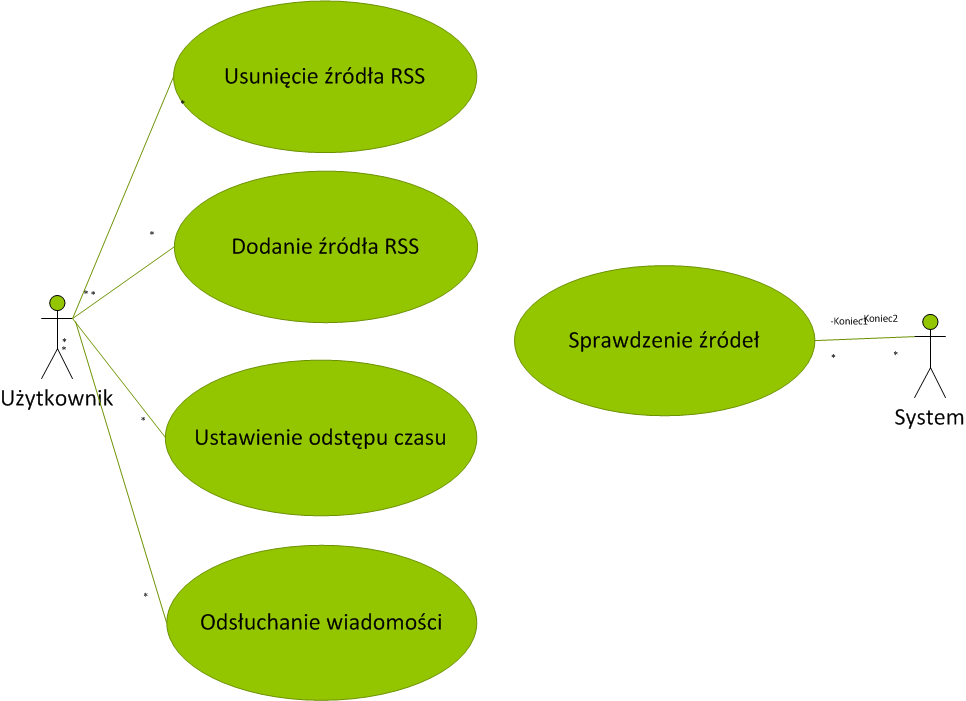
\includegraphics[scale=0.45]{useCaseRSS.png} 
	\caption{Przypadek użycia - LektorRSS}
\end{figure}

\subsubsection{Wymagania funkcjonalne}
\begin{enumerate}
	\item Możliwość dodania źródła RSS
	\item Możliwość usunięcia źródła RSS
	\item Obsługiwanie więcej niż jednego języka wiadomości
	\item Automatyczne sprawdzanie czy któreś ze źródeł nie zawiera nowej wiadomości
	\item Możliwość ustawienia odstępów czasowych pomiędzy sprawdzaniem przez system źródeł
	\item Automatyczne Odczytanie użytkownikowi nowych wiadomości (w przypadku istnienia) 
\end{enumerate}  
\subsubsection{Wymagania niefunkcjonalne}
\begin{enumerate}
	\item Niezawodność - system nie może pominąć żadnej wiadomości z listy źródeł zdefiniowanej przez użytkownika
	\item Szybkość - różnica czasu pomiędzy udostępnieniem nowej wiadomości w którymś ze źródeł a otrzymaniem jej przez użytkownika nie może przekraczać czasu pomiędzy sprawdzeniami w poszukiwaniu uaktualnień (czas ten ustawia użytkownik)
	\item Możliwość personalizacji - użytkownik powinien móc dodać dowolną ilość różnych źródeł, system powinien zapewnić ich niepowtarzalność(usuwać duplikaty)
\end{enumerate}

\subsubsection{Weryfikacja podejścia}
Tak jak w sekcji opisującej aplikację Automatyczne Dyktando wymagania przedstawione powyżej są jasne i klarowne. Po raz kolejny zastosowane podejście integracyjne sprawia, że napisanie aplikacji klienckiej, spełniającej wymagania przed nią stawiane jest proste. Dzięki użyciu ESB i oferowanych przez niego punktów końcowych jest możliwe przerzucenie konieczności pobierania wiadomości ze źródeł RSS na stronę systemu. Podobnie jak w przypadku aplikacji opisanej wyżej zarówno rozpoznawanie języka, tłumaczenie czy generowanie mowy w odpowiednim języku nie stanowi dla programisty, autora aplikacji klienckiej, żadnego problemu, wystarczającym jest wygenerowanie pliku xml zawierającego odpowiednie instrukcje. Implementacja podobnej, równie rozbudowanej aplikacji, bez wykorzystania systemu integrującego usługi odpowiadające za przetwarzanie mowy, byłaby trudniejsza oraz wymagałaby poświęcenia większej ilości czasu. Poza problemami podobnymi do tych jakie były opisane w przypadku Automatycznego Dyktanda dochodzi jeszcze sprawa pobierania wiadomości RSS, ich parsowania itd. Pozostałe wymagania, takie jak bezpieczeństwo czy też konieczność przechowywania danych w bazie danych muszą być zaspokojone w ten sam sposób niezależnie od wykorzystania systemu. \\
W przypadku tej aplikacji również klarownym jest fakt, że zastosowane podejście bardzo upraszcza implementację.

\section{Weryfikacja wydajności}
W części tej opisane są wyniki testów jak i testy którym został poddany prototyp platformy oraz ich porównanie z wynikami testów przeprowadzonych bezpośrednio na integrowanych usługach.
\subsection{Usługa TTS}
Test dla usługi TTS polegał na syntezie tekstu  w języku angielskim, zamieszczonego na rysunku\ref{fig:ttsExample}.
\begin{figure}[!h]
\centering
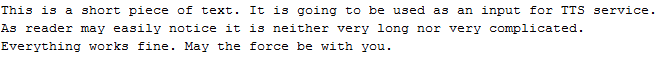
\includegraphics[scale=0.9]{textExample.png}
\caption{Przykładowy tekst dla usługi TTS}\label{fig:ttsExample}
\end{figure}
Ponieważ w obu przypadkach wykorzystano ten sam tekst jakość odczytu była taka sama. Jedyna różnica występuje w czasie działania. Próbę powtórzono dziesięciokrotnie, wyniki można zaobserwować w tabeli \ref{tab:tts}. Należy zaznaczyć, że ''Web service'' oznacza bezpośrednie wywołanie usługi TTS, a ''Prototyp'' wywołanie usługi poprzez przykładową implementację platformy integracyjnej.
\begin{center}
	\begin{table}[h]
	\caption{Test TTS}
	\label{tab:tts}
	\centering
	\begin{tabular}{| l | l | l |}	
		\hline
		\textbf{Numer testu} & \textbf{Web service [ms]} & \textbf{Prototyp [ms]} \\ \hline
		1 & 1332 & 1476\\ \hline
		2 & 1376 & 1493\\ \hline
		3 & 1241 & 1387\\ \hline
		4 & 1250 & 1315\\ \hline
		5 & 1236 & 1489\\ \hline
		6 & 1225 & 1424\\ \hline
		7 & 1288 & 1398\\ \hline
		8 & 1234 & 1503\\ \hline
		9 & 1184 & 1131\\ \hline
		10 & 1230 & 1543\\ \hline
		\textbf{Średnia/Odchylenie standardowe} & 1256.6/145.182 & 1415.9/84.14\\ 
		\hline
	\end{tabular}
	\end{table}
\end{center}
Jak łatwo można zaobserwować koszt czasowy użycia prototypowego systemu nie jest duży. Co więcej jest on stabilny, nie odnotowano wystąpień dużych odchyleń. 

\subsection{Usługa Translacji}
Test dla usługi translacji polegał na tłumaczeniu tekstu z języka polskiego na język angielski. Tekst który posłużył nam w tym teście został zamieszczony na rysunku \ref{fig:translatorExample}.
\begin{figure}[!h]
\centering
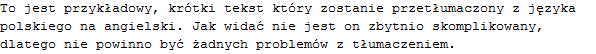
\includegraphics[scale=0.9]{translatorExample.png}
\caption{Przykładowy tekst dla usługi translacji}\label{fig:translatorExample}
\end{figure}
Ponieważ użyto tej samej usługi tłumaczącej jego efekt za każdym razem był taki sam. Rysunek \ref{fig:translatorResult} przedstawia tekst wynikowy, efekt można uznać za zadowalający acz nie bezbłędny. 
\begin{figure}[!h]
\centering
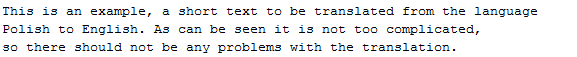
\includegraphics[scale=0.9]{translatorResult.png}
\caption{Wynik translacji}\label{fig:translatorResult}
\end{figure}

Próbę powtórzono dziesięciokrotnie, wyniki można zaobserwować w tabeli \ref{tab:translacja}. Należy zaznaczyć, że ''Web service'' oznacza bezpośrednie wywołanie usługi translacji, a ''Prototyp'' wywołanie usługi poprzez przykładową implementację platformy integracyjnej.
\begin{center}
	\begin{table}[h]
	\centering
	\begin{tabular}{| l | l | l |}	
		\hline
		\textbf{Numer testu} & \textbf{Web service [ms]} & \textbf{Prototyp [ms]} \\ \hline
		1 & 618 & 560\\ \hline
		2 & 477 & 801\\ \hline
		3 & 433 & 546\\ \hline
		4 & 407 & 593\\ \hline
		5 & 390 & 550\\ \hline
		6 & 437 & 774\\ \hline
		7 & 645 & 683\\ \hline
		8 & 430 & 501\\ \hline
		9 & 394 & 578\\ \hline
		10 & 410 & 618\\ \hline
		\textbf{Średnia/Odchylenie standardowe} & 464.1/38.01645 & 620.4/41.7235\\ 
		\hline
	\end{tabular}
	\caption{Test Translacji}
	\label{tab:translacja}
	\end{table}
\end{center}
Koszt czasowy wykorzystania prototypu nie jest duży, co więcej nie odnotowano wystąpień dużych odchyleń, co świadczy o stabilności.

\subsection{Usługa OCR}
Test dla usługi OCR polegał na rozpoznawaniu tekstu znajdującego się na obrazku w formie jpg, obrazek jest przedstawiony na rysunku \ref{fig:OCRExample}. 
\begin{figure}[!h]
\centering
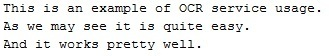
\includegraphics[scale=0.9]{OCRExample.jpg}
\caption{Plik wejściowy dla usługi OCR}\label{fig:OCRExample}
\end{figure}
Ponieważ użyto tej samej usługi OCR jego efekt za każdym razem był taki sam. Rysunek \ref{fig:OCRResult} przedstawia tekst wynikowy, efekt można uznać za bezbłędny acz należy wziąć pod uwagę prostotę tego przykładu.
\begin{figure}[!h]
\centering
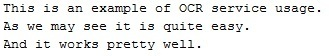
\includegraphics[scale=0.9]{OCRExample.jpg}
\caption{Wynik działania usługi OCR}\label{fig:OCRResult}
\end{figure}
Próbę powtórzono dziesięciokrotnie, wyniki można zaobserwować w tabeli \ref{tab:ocr}. Należy zaznaczyć, że ''Web service'' oznacza bezpośrednie wywołanie usługi OCR, a ''Prototyp'' wywołanie usługi poprzez przykładową implementację platformy integracyjnej.
\begin{center}
	\begin{table}[h]
	\centering
	\begin{tabular}{| l | l | l |}	
		\hline
		\textbf{Numer testu} & \textbf{Web service [ms]} & \textbf{Prototyp [ms]} \\ \hline
		1 & 2961 & 3712\\ \hline
		2 & 3509 & 5486\\ \hline
		3 & 4427 & 4135\\ \hline
		4 & 5258 & 4444\\ \hline
		5 & 3929 & 4052\\ \hline
		6 & 3641 & 3084\\ \hline
		7 & 4012 & 4550\\ \hline
		8 & 4321 & 3632\\ \hline
		9 & 5363 & 5381\\ \hline
		10 & 3589 & 3764\\ \hline
		\textbf{Średnia/Odchylenie standardowe} & 4101/472.1354 & 4224/457.2335\\ 
		\hline
	\end{tabular}
	\caption{Test OCR}
	\label{tab:ocr}
	\end{table}
\end{center}
Koszt czasowy wykorzystania prototypu nie jest duży, co więcej nie odnotowano wystąpień dużych odchyleń, co świadczy o stabilności. 

\subsection{Test złożony}
Celem tego testu było wypróbowanie bardziej złożonego scenariusza jakim jest wysłanie do prototypowej implementacji systemu pliku graficznego wraz z plikiem konfiguracyjnym xml przedstawionym na rysunku \ref{fig:xmlConf}.
\begin{figure}[!h]
\centering
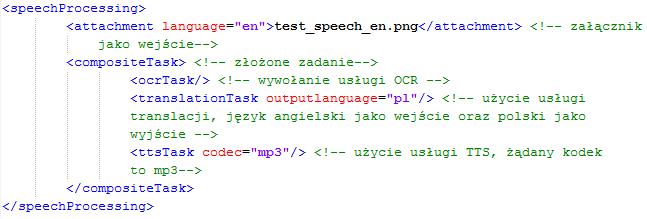
\includegraphics[scale=0.9]{xmlConf.png}
\caption{Plik konfiguracyjny xml}\label{fig:xmlConf}
\end{figure}
W jego wyniku otrzymano plik dźwiękowy w formacie mp3, zawierający odczyt tekstu będącego tłumaczeniem tekstu znajdującego się na obrazku \ref{fig:OCRExample} wysłanym na wejście. Gdyby zapisać zdania czytane przez lektora wyglądałyby one następująco: ''To jest przykład użycia OCR usług. Jak możemy zobaczyć, jest to dość proste. I to działa całkiem dobrze.''. Nie stwierdzono żadnych niewyraźnie przeczytanych wyrazów, ani innych nieprawidłowości. Tłumaczenie również jest całkiem poprawne. Test powtórzono dziesięciokrotnie, wyniki są zaprezentowane w tabeli \ref{tab:bigTest}. Należy zaznaczyć, że ''Web service'' oznacza bezpośrednie wywołanie usług, a ''Prototyp'' wywołanie tych samych usług poprzez przykładową implementację platformy integracyjnej.
\begin{center}
	\begin{table}[t]
	\caption{Test złożony}
	\label{tab:bigTest}
	\centering
	\begin{tabular}{| l | l | l |}	
		\hline
		\textbf{Numer testu} & \textbf{Web services [ms]} & \textbf{Prototyp [ms]} \\ \hline
		1 & 4911 & 5552\\ \hline
		2 & 5362 & 7264\\ \hline
		3 & 6101 & 6308\\ \hline
		4 & 6915 & 6268\\ \hline
		5 & 5555 & 5626\\ \hline
		6 & 5303 & 5878\\ \hline
		7 & 5945 & 7238\\ \hline
		8 & 5985 & 6424\\ \hline
		9 & 6941 & 5685\\ \hline
		10 & 5229 & 5234\\ \hline
		\textbf{Średnia/Odchylenie standardowe} & 5824.7/843.4343 & 6147.7/823.7793\\ 
		\hline
	\end{tabular}
	\end{table}
\end{center}
\newpage
Jako czas potrzebny na wykonanie scenariusza w przypadku bezpośredniego wywołania usług wzięto sumę czasów potrzebnych do wywołania każdej z osobna. W przypadku wykorzystania prototypowego systemu czas wykonania zadania nie jest znacząco większy niż przy bezpośrednim wywołaniu usług. Co więcej jest on mniejszy niż gdyby zsumować czas potrzebny na wywołanie każdej z usług osobno za pomocą platformy. Prawdopodobnie wynika to z faktu, że przy wywołaniu złożonego scenariusza mamy tylko jedno zapytanie na drodze klient - platforma, zamiast trzech które byłyby potrzebne do wywołania każdej usługi osobno.  

\section{Wnioski}
Jak widać zastosowanie prototypowej platformy wprowadza pewien narzut czasowy, nie jest on jednak duży. W zamian klient takiej usługi otrzymuje znacznie prostszy interfejs, który mimo swojej prostoty daje duże możliwości. Co więcej klient nie musi martwić się o potencjalne błędy, konwersje między formatami, niedostępność którejś z usług składowych itd. Podsumowując, zastosowanie takiej platformy jest uzasadnione, jest ona funkcjonalna, nie wprowadza opóźnień oraz posiada szeroki zakres usług. 
% ---------------------------------------------------------------------------
%: ----------------------- end of thesis sub-document ------------------------
% ---------------------------------------------------------------------------

